
%(BEGIN_QUESTION)
% Copyright 2007, Tony R. Kuphaldt, released under the Creative Commons Attribution License (v 1.0)
% This means you may do almost anything with this work of mine, so long as you give me proper credit

Explain what a {\it first-order} process is.

\underbar{file i01679}
%(END_QUESTION)





%(BEGIN_ANSWER)

A first-order process is one having a single mode of storage (either of energy or of matter) and ``resistive'' element limiting the rate at which the storage element may be filled or unfilled.  This leads to behavior like that of a simple RC circuit.  In fact, first-order processes may be electrically simulated using nothing but a single capacitor and a single resistor.

%(END_ANSWER)





%(BEGIN_NOTES)

The energy storage in the process may be thermal, inertial, or even chemical.  ``Resistance'' in the process is anything impeding the immediate and unrestricted storage or release of energy.

\vskip 10pt

A classic example of a first-order process is a discharging capacitor:

$$\includegraphics[width=15.5cm]{i01679x01.eps}$$

The fundamental equations in this circuit are:

$$i = {v \over R} \hbox{\hskip 50pt} i = C {dv \over dt}$$

Recognizing that the current for both of these components ($R$ and $C$) are equal and opposite in direction:

$$C {dv \over dt} = - {v \over R}$$

Solving this separable differential equation:

$${dv \over dt} = - {v \over RC}$$

$${1 \over v} \> dv = - {1 \over RC} \> dt$$

$$\int {1 \over v} \> dv = \int -{1 \over RC} \> dt$$

$$\int {1 \over v} \> dv = - {1 \over RC} \int \> dt$$

$$\ln |v| + k_1 = - {1 \over RC} t + k_2$$

$$\ln |v| = - {t \over RC} + k_3$$

$$|v| = e^{(- {t \over RC} + k_3)}$$

$$|v| = e^{(- {t \over RC})} e^{k_3}$$

$$|v| = k_4 e^{(- {t \over RC})}$$

$$v = k e^{(- {t \over RC})}$$

$$v = V_0 e^{(- {t \over RC})}$$

%INDEX% Control, basics: first-order process response

%(END_NOTES)


